\chapter{Влияние шероховатой поверхности на кинетические эффекты в низкоразмерных системах} \label{chapt3}

\section{ Подвижность носителей в размерно-квантованных системах с учетом рассеяния на поверхности и фононах}

Квантовые системы с пониженной размерностью (квантовые ямы (КЯ), сверхрешетки, квантовые проволоки (КП)) благодаря их уникальным свойствам, связанным с возникновением размерного квантования, продолжают привлекать внимание теоретиков и экспериментаторов. При этом кинетические явления в размерно-квантованных системах принципиальным образом отличаются от объемных материалов. Так, например, в объемных материалах сопротивление растет с увеличением температуры T, а в КП малого диаметра d ($d \sim 70 \AA$) убывает, оставаясь практически постоянным в области низких T \cite{Lin2000,Lin2003,Heremans1998,Zhang2000,Heremans2000}. Для КЯ GaAs/AlAs температурная зависимость подвижности $\mu (T)$ может носить не монотонный характер: в области низких температур (T$>$10K) $\mu (T)$ увеличивается с ростом T, а при T$>$100K начинает уменьшаться \cite{Lin2000,Sakaki1987}. Следовательно, размеры квантовых систем принципиальным образом могут влиять на величину и температурную зависимость электропроводности.

В данной диссертационной работе делается попытка объяснить особенности температурной зависимости электропроводности, экспериментально наблюдаемые в нелегированных наноструктурах, учитывая процессы рассеяния носителей на шероховатой поверхности и на фононах. Именно из сравнения теоретических результатов с экспериментальными данными по температурной зависимости электропроводности можно провести оценки параметров флуктуирующей поверхности. Учет двух механизмов рассеяния позволил сформулировать условия на ширину размерно-ограниченной системы и температуру, когда рассеяние электронов на фононах преобладает над поверхностным рассеянием.

Расчет электропроводности проводится согласно формуле Кубо \cite{Kubo1957a} для статической электропроводности, которая в представлении вторичного квантования имеет вид\footnote{ Полученное выражение для электропроводности справедливо для любых квантовых систем в произвольном магнитном поле. Единственное ограничение -- это малость электрического поля, т.е. область применимости закона Ома.}:
\begin{equation} \label{eq:31_10}
\sigma _{ij} =\frac{\beta _{0} e^{2} }{2Vm^{2} } \sum _{\alpha ,\beta ,\alpha _{1} ,\beta _{1} }\hat{p}_{\alpha \beta }^{(i)} \hat{p}_{\alpha _{1} \beta }^{(j)} \int _{-\infty }^{\infty }dt\left\langle a_{\alpha }^{+} (t)a_{\beta } (t)a_{\alpha _{1} }^{+} a_{\beta _{1} } \right\rangle
\end{equation} 
$\hat{p}_{\alpha \beta }^{(i)} $ -- матричный элемент оператора импульса на сглаженных волновых функциях зонного электрона, $\beta _{0} =1/k_{0} T$, $\alpha $ -- квантовые числа, описывающие состояние заряженной частицы с эффективной массой m, $V$ -- объем основной области системы,
\[
a_{\alpha }^{+} (t)={\mathrm exp}\left(\frac{it\hat{H}}{\hbar } \right)a_{\alpha }^{+} {\mathrm exp}\left(-\frac{it\hat{H}}{\hbar } \right),
\] 
$\left\langle \cdot \cdot \cdot \right\rangle $ -- описывает усреднение по системе равновесных электронов и по реализации случайного процесса

Гамильтониан для электрона, взаимодействующего с шероховатой поверхностью размерно-ограниченной системы в представлении вторичного квантования записывается в виде:
\begin{equation} \label{eq:31_20}
\hat{H}=\sum _{\alpha }\varepsilon _{\alpha } a_{\alpha }^{+} a_{\alpha } +\sum _{\alpha ,\beta }{\left\langle \alpha  \right|} \hat{V}{\left| \beta  \right\rangle} a_{\alpha }^{+} a_{\beta }, 
\end{equation}
$\hat{V}$ -- оператор взаимодействия носителя с энергией $\varepsilon _{\alpha } $ с поверхностью системы, ${\left| \alpha  \right\rangle} $ -- волновая функция зонного электрона.

Если учесть временную зависимость операторов рождения уничтожения (\dots .) в \eqref{eq:31_10}, то после усреднения с матрицей плотности удовлетворяющей уравнению нейтральности с гамильтонианом ${\hat{H}}_0$ не трудно получить:
\begin{multline} \label{eq:31_30}
{\sigma }_{ij}=\frac{{\beta }_0 e^2}{2Vm^2_e}\sum_{\alpha \alpha _1\beta \beta_1}{{\hat{P}}^{\left(i\right)}_{\alpha {\alpha }_1}{\hat{P}}^{\left(j\right)}_{\beta {\beta }_1}n_{{\beta }_1}\left(1-n_{\beta }\right)}\\
\int^{\infty }_{-\infty }{d t {\left\{\left\langle {\beta }_1\left|e^{\frac{it}{\hbar }\left(H_0+V\right)}\right|\alpha \right\rangle \left\langle {\alpha }_1\left|e^{\frac{i t}{\hbar }\left(H_0+V\right)}\right|\beta \right\rangle \right\}}_V}
\end{multline}

\noindent ${\left\{\cdots \right\}}_V$~---~описывает усреднение по реализации случайного процесса $\Delta \left(x,y\right)$, $n_{\beta }$~---~равновесная функция распределения Ферми-Дирака для электронов с энергией $E_{\alpha }$ .

В дальнейшем проведем усреднение для матричных элементов в \eqref{eq:31_30} независимо. {\color{red}Такое приближение соответствует приближению «времени релаксации» [x.]} и конечные результаты для кинетических коэффициентов будут вероятно отличаться от тех, которые получаются при использовании решения классического уравнения Больцмана. Далее этот вопрос будет детально обсуждать ниже.

\noindent Рассмотрим функцию
\begin{multline} \label{eq:31_40}
y_{{\beta }_1\alpha }=e^{-\frac{it}{\hbar }E_{{\beta }_1}}{\left\{\left\langle {\beta }_1\left|e^{\frac{it}{\hbar }\left(H_0+V\right)}\right|\alpha \right\rangle \right\}}_V=\\
={\left\{\left\langle {\beta }_1\left|T{{\exp}_{[-]} \left[\frac{i}{\hbar }\int^{\infty }_0{V\left(\tau \right)d \tau }\right]\ }\right|\alpha \right\rangle \right\}}_V
\end{multline}

\noindent Здесь обозначено
\[
T{{\exp}_{\left[-\right]} \left[\frac{i}{\hbar }\int^{\infty }_0{V\left(\tau \right)d \tau }\right]\ }=e^{-\frac{it}{\hbar }H_0}e^{\frac{it}{\hbar }\left(H_0+V\right)},\ \ V\left(\tau \right)=e^{-\frac{i\tau }{\hbar }H_0}Ve^{\frac{i\tau }{\hbar }\left(H_0\right)}
\] 
{\color{red}Усреднение по реализации случайного процесса в \eqref{eq:31_40} проведем с использованием кумулянтного усреднения [???].} В результате до второй кумулянты \eqref{eq:31_40} принимает следующий вид:
\begin{equation} \label{eq:31_50}
y_{{\beta }_1\alpha }\left(t\right)=\left\langle {\beta }_1\left|{exp \left\{-\frac{1}{{\hbar }^2}\int^t_0{d \tau \int^{\tau }_0{d {\tau }_1{\left\{V\left({\tau }_1\right)V\left(\tau \right)\right\}}_V}}\right\}\ }\right|\alpha \right\rangle
\end{equation} 

\noindent Не трудно показать, что
\begin{equation} \label{eq:31_60}
{\dot{y}}_{{\beta }_1\alpha }\left(t\right)=-\frac{1}{{\hbar }^2}\int^t_0{d \tau \sum_{\gamma }{\left\langle {\beta }_1\left|{\left\{V\left({\tau }_1\right)V\left(t\right)\right\}}_V\right|\gamma \right\rangle y_{\gamma \alpha }\left(t\right)}}
\end{equation} 

\noindent Дальнейшие расчеты проводятся в диагональном приближении, так как процессы рассеяния носителей на шероховатой поверхности являются упругими и происходят в основном в одной размерно-квантованной зоне проводимости. Решение дифференциального уравнения \eqref{eq:31_60} в диагональном приближении $\gamma ={\beta }_1$ с начальным условием $y_{{\beta }_1\alpha }\left(0\right)={\delta }_{{\beta }_1\alpha }$ записывается следующим образом:
\begin{equation} \label{eq:31_70}
y_{{\beta }_1\alpha }\left(t\right)=\exp \left\{-\frac{1}{{\hbar }^2}\int^t_0{d \tau \int^{\tau }_0{d {\tau }_1\left\langle {\beta }_1\left|{\left\{V\left(\tau \right)V\left({\tau }_1\right)\right\}}_V\right|{\beta }_1\right\rangle }}\right\}{\delta }_{{\beta }_1\alpha }
\end{equation} 

\noindent Не трудно показать (см. \S 2 гл. 1), что
\begin{equation} \label{eq:31_80}
\left\langle {\beta }_1\left|{\left\{V\left(\tau \right)V\left({\tau }_1\right)\right\}}_V\right|{\beta }_1\right\rangle =\sum_{\gamma }{W_{{\beta }_1\gamma }\exp \left[\frac{i}{\hbar }\left({\tau }_1-\tau \right)\left({\varepsilon }_{{\beta }_1}-{\varepsilon }_{\gamma }\right)\right]\ }
\end{equation} 

\noindent Если подставить \eqref{eq:31_70} в \eqref{eq:31_60} и провести интегрирование по $\tau ,{\tau }_1$, в результате получаем

\begin{equation} \label{eq:31_90}
y_{{\beta }_1\alpha }\left(t\right)=\exp \left\{g_{\alpha }\left(t\right)\right\}{\delta }_{{\beta }_1\alpha}
\end{equation}

\begin{multline} \label{eq:31_100}
g_{\alpha }\left(t\right)=-2\sum_{\gamma }{W_{\alpha \gamma }\frac{{{\sin}^2 \frac{t}{\hbar }\left({\varepsilon }_{\alpha }-{\varepsilon }_{\gamma }\right)\ }}{{\left({\varepsilon }_{\alpha }-{\varepsilon }_{\gamma }\right)}^2}}+\\
+i\sum_{\gamma }{\frac{W_{\alpha \gamma }}{\left({\varepsilon }_{\alpha }-{\varepsilon }_{\gamma }\right)}}\left\{\frac{t}{\hbar }-\frac{1}{\left({\varepsilon }_{\alpha }-{\varepsilon }_{\gamma }\right)}{\sin \frac{t}{\hbar }\left({\varepsilon }_{\alpha }-{\varepsilon }_{\gamma }\right)\ }\right\} \notag	
\end{multline}

\noindent Первое слагаемое в $g_{\alpha }\left(t\right)$ связано с квантово-механической вероятностью перехода носителя под влиянием возмущения $V$ [???]; второе слагаемое, в частности, определяет изменение энергии электрона под влиянием возмущения $V$.

\noindent Если \eqref{eq:31_90} и $y_{{\alpha }_1\beta }\left(\_t\right)$ подставить в \eqref{eq:31_30}, то электропроводность можно записать в виде
\begin{equation} \label{eq:31_110}
{\sigma }_{ij}=\frac{{\beta }_0e^2}{2Vm^2_e}\sum_{\alpha \beta }{{\hat{P}}^{\left(i\right)}_{\alpha \beta }{\hat{P}}^{\left(j\right)}_{\beta \alpha }n_{\alpha }\left(1-n_{\beta }\right)}\int^{\infty }_{-\infty }{d te^{\frac{it}{\hbar }\left({\varepsilon }_{\alpha }-{\varepsilon }_{\beta }\right)}\exp \left[g_{\alpha }\left(t\right)+g_{\beta }\left(\_t\right)\right]}
\end{equation} 

\noindent Если рассматривать упругое рассеяние в одной зоне и учесть, что в дальнейшем рассматриваем кинетические процессы с ${\hat{P}}_{\alpha \beta }\sim {\delta }_{\alpha \beta }$, то \eqref{eq:31_110} можно представить в виде $(i=j)$:

\begin{multline} \label{eq:31_120}
{\sigma }_{ij}=\frac{{\beta }_0e^2}{2Vm^2_e}\sum_{\alpha }{{\left|{\hat{P}}^i_{\alpha \alpha }\right|}^2 n_{\alpha }\left(1-n_{\alpha }\right)}\\
\int^{\infty }_{-\infty }{d t{\exp \left[-\sum_{\gamma }{W_{\alpha \gamma }\frac{4{{\sin}^2 \frac{t}{\hbar }\left({\varepsilon }_{\alpha }-{\varepsilon }_{\gamma }\right)\ }}{{\left({\varepsilon }_{\alpha }-{\varepsilon }_{\gamma }\right)}^2}}\right]}}
\end{multline}

\noindent При $t\to \infty $, {\color{red}когда можно ввести понятие о независящей от времени вероятности перехода [???]}, то

\begin{equation} \label{eq:31_130}
\sum_{\gamma }{W_{\alpha \gamma }\frac{4{{\sin}^2 \frac{t}{\hbar }\left({\varepsilon }_{\alpha }-{\varepsilon }_{\gamma }\right)\ }}{{\left({\varepsilon }_{\alpha }-{\varepsilon }_{\gamma }\right)}^2}}\Rightarrow \left|t\right|\frac{1}{{\tau }_{\alpha }};
\end{equation}
 
\begin{equation} \label{eq:31_140}
\frac{1}{{\tau }_{\alpha }}=\sum_{\gamma }{W_{\alpha \gamma }\delta \left({\varepsilon }_{\alpha }-{\varepsilon }_{\gamma }\right)}
\end{equation}


\noindent ${1}/{{\tau }_{\alpha }}$ -- квантово-механическая вероятность рассеяния носителей на шероховатой поверхности.

 С учетом \eqref{eq:31_130} электропроводность определяется соотношением

\begin{equation} \label{eq:31_150}
{\sigma }_{ij}=\frac{{\beta }_0e^2}{Vm^2_e}\sum_{\alpha }{{\left|{\hat{P}}^i_{\alpha \alpha }\right|}^2n_{\alpha }\left(1-n_{\alpha }\right)}{\tau }_{\alpha }
\end{equation}

\noindent Заметим, что соотношение для электропроводности \eqref{eq:31_150} получено из самых общих соотношений квантовой статистики без привлечения решения классического уравнения Больцмана, которое, как известно имеет ограниченную область применения. В классическое выражение для тензора электропроводности входит не время релаксации ${\tau }_{\alpha }$, а транспортное время релаксации, которое естественным образом возникает при решении кинетического уравнения Больцмана \cite{Anselm1978}. При этом время релаксации и транспортное время в случае упругого рассеяния носителей на длинноволновых акустических колебаниях, на примесях, при рассеянии на шероховатой поверхности в случае $\delta $-образной флуктуации поверхности не отличаются. (В случае гауссовой флуктуации поверхности см. замечание в \S 2 гл.1) Последнее обстоятельство является не случайным, т.к. выражение для электропроводности \eqref{eq:31_150} получено при условии упругих процессов рассеяния носителей и при возможности введения независимой от времени вероятности процесса рассеяния. Но именно из тех же соображений вводится интеграл столкновений при выводе классического уравнения Больцмана.

Для прямоугольной КЯ с бесконечным потенциалом для случая гауссовой флуктуации поверхности

\begin{equation} \label{eq:31_160}
W_{\gamma \beta } =\frac{\pi }{L_{x} L_{y} } (\Delta \Lambda )^{2} V_{\gamma } V_{\beta } {\mathrm exp}\left[-\frac{\Lambda ^{2} }{4} \left|k_{\bot } -k'_{\bot } \right|^{2} \right],
\end{equation}

\noindent и время релаксации при рассеянии носителей в одной зоне определяется соотношением:

\begin{equation} \label{eq:31_170}
\frac{1}{\tau _{\alpha } } =\frac{\pi m(\Delta \Lambda V_{1} )^{2} }{\hbar ^{3} } {\mathrm exp}\left(-\frac{\Lambda ^{2} }{2} k_{\bot }^{2} \right){\mathrm I}_{{\mathrm 0}} \left(\frac{\Lambda ^{2} }{2} k_{\bot }^{2} \right),   (10)
\end{equation}

\noindent ${\mathrm I}_{0} (z)$ -- модифицированная функция Бесселя нулевого индекса, $V_{1} =-\frac{\hbar ^{2} \pi ^{2} }{mL^{3} } $.

Рассмотрим, случай, когда электроны находятся на нижайшем размерно-квантованном уровне ($n=1$) прямоугольной КЯ. Это выполнимо, если $3\hbar ^{2} \pi ^{2} /\left(2mL^{2} \right)>>k_{0} T$. В результате \eqref{eq:31_150} после суммирования по $k_{\bot } $ принимает вид:

\begin{equation} \label{eq:31_180}
\sigma _{xx} =\frac{e^{2} \hbar ^{3} }{m^{2} \pi ^{2} \left(\Delta \Lambda ^{2} V_{1} \right)^{2} L} \delta \int _{0}^{\infty }d\tau \frac{\tau \cdot {\mathrm exp}\left(\delta \tau -\beta \tilde{\xi }\right)}{{\mathrm exp(}-\tau ){\mathrm I}_{{\mathrm 0}} (\tau )\cdot \left[{\mathrm exp}\left(\delta \tau -\beta \tilde{\xi }\right)+1\right]^{2} },
\end{equation}

\[
\delta =\frac{\beta _{0} \hbar ^{2} }{m_{e} \Lambda ^{2} },
\] 

$\tilde{\xi }=\xi -\varepsilon _{1} $ -- химический потенциал, отсчитанный от дна нижайшей зоны:

\begin{equation} \label{eq:31_190}
\beta _{0} \tilde{\xi }={\mathrm ln}\left[{\mathrm exp}\left(\frac{\beta _{0} \pi \hbar ^{2} n_{s} }{m} \right)-1\right].
\end{equation}

\noindent  $n_{s} $~---~поверхностная плотность электронного газа.

Для невырожденного электронного газа

$$\left(\beta _{0} \pi \hbar ^{2} n_{s} /m_{e} <<1\right), {\exp}\left(\beta _{0} \tilde{\xi }\right)=\beta _{0} \pi \hbar ^{2} n_{s} /m_{e}, $$

\noindent и согласно \eqref{eq:31_180} нетрудно вычислить подвижность:

\begin{equation} \label{eq:31_200}
\mu ^{(nd)} =\mu _{0} \delta ^{2} \int _{0}^{\infty }d\tau \frac{\tau \cdot \exp \left[-\left(\delta -1\right)\tau \right]}{I_{0} (\tau )},
\end{equation}

\[
\mu _{0} =\frac{e}{\hbar \pi ^{5} } \left(\frac{L^{3} }{\Delta \Lambda } \right)^{2}.
\] 

Следовательно, подвижность существенным образом зависит от толщины размерно-квантованной системы $(\mu _{0} \sim L^{6} )$. На рис. 1a (кривая 1) приведена температурная зависимость $\mu ^{(nd)} /\mu _{0} $ с учетом зависимости химического потенциала от температуры \eqref{eq:31_190}. Как непосредственно следует из рис. 1a при низких $T$ $(\delta >>1)$ подвижность практически не зависит от температуры и при высоких температурах $(\delta <1)$ с ростом T увеличивается (кривая 1). Такое поведение подвижности от L и T экспериментально наблюдалось в GaAs/AlAs \cite{Sakaki1987}. При низких температурах $\mu ^{(nd)} =\mu _{0} $, т.е. определяется только размером КЯ и параметрами флуктуирующей поверхности $\Delta $, $\Lambda $. При изменении толщины КЯ от $70 \AA$ до $100 \AA$ подвижность изменяется от $\mu _{0} =2.6\cdot 10^{3} \text{cm}^{2} /{Vs}$ до $\mu _{0} =2\cdot 10^{4} \text{cm}^{2} /{Vs}$, что согласуется с экспериментальными данными в КЯ GaAs/AlAs \cite{Sakaki1987}.

Для вырожденного электронного газа при низких T электропроводность принимает вид:

\begin{equation} \label{eq:31_210}
\sigma _{xx}^{(d)} =\frac{e^{2} \hbar \tilde{\xi }}{\pi ^{2} Lm\left(\Delta \Lambda V_{1} \right)^{2} } \frac{{\mathrm exp}\left(\frac{m\Lambda ^{2} }{\hbar ^{2} } \tilde{\xi }\right)}{{\mathrm I}_{{\mathrm 0}} \left(\frac{m\Lambda ^{2} }{\hbar ^{2} } \tilde{\xi }\right)} ,    (14)
\end{equation}


Если $\beta _{0} \pi \hbar ^{2} n_{s} /m>>1$, то $\tilde{\xi }=\pi \hbar ^{2} n_{s} /m$ и подвижность определяется соотношением:

\begin{equation} \label{eq:31_220}
\mu ^{(d)} =\mu _{0} \frac{{\mathrm exp}\left(a\right)}{{\mathrm I}_{{\mathrm 0}} \left(a\right)},
\end{equation}

\[
a=\pi \Lambda ^{2} n_{s}
\]

При $a<<1$ 

\begin{equation} \label{eq:31_230}     
\mu ^{(d)} =\mu _{0}.
\end{equation}

При $a>>1$

\begin{equation} \label{eq:31_240}  
\mu ^{(d)} =\mu _{0} \pi \sqrt{2\Lambda ^{2} n_{s} }
\end{equation}

Как следует из \eqref{eq:31_230} в исследуемой модели КЯ подвижность в области низких температур не зависит от T (кривая 2 на рис. a). Такое поведение $\mu ^{(d)} $ от $T$ экспериментально наблюдалось в кремниевых инверсионных слоях, в которых электронный газ остается вырожденным вплоть до $T<100 K$ ($\tilde{\xi }=12.5 \text{meV}$, $n_{s} =2\cdot 10^{12} \text{cm}^{-2} $) \cite{Stern1980}. Для $\Delta =6\AA$, $\Lambda =13 \AA$, при $L=70 \AA$, $n_{s} =2\cdot 10^{12}  \text{cm}^{-2} $ ($a<<1$) $\mu ^{d} =1.5\cdot 10^{4} \text{cm}^{2} /{Vs}$, что близко к экспериментальным данным \cite{Stern1980}.

Аналогичные расчеты подвижности можно провести для прямоугольной квантовой ямы при $\delta $-образной флуктуации поверхности. Учитывая предельный переход от гауссовой флуктуации поверхности к $\delta $-образной, когда $\Lambda \to 0$, ${\left(\Delta \Lambda \right)}^2\to \pi \gamma $ (см. замечание в параграфе 2 гл. 1) не трудно получить выражение для электропроводности. Согласно \eqref{eq:31_180} электропроводность в этом случае может быть записана в виде:

\begin{equation} \label{eq:31_250}
{\sigma }^{\delta }_{xx}=\frac{e^2\hbar }{{\pi }^3{\beta }_0m_eLV^2_1\gamma }\int^{\infty }_0{\frac{xd xe^{x-\beta \widetilde{\xi }}}{{\left(e^{x-\beta \widetilde{\xi }}+1\right)}^2}}
\end{equation} 

\noindent Для случая невырожденного газа из \eqref{eq:31_250} нетрудно получить выражения для подвижности

\begin{equation} \label{eq:31_260}
{\mu }^{\delta \left(nd\right)}=\frac{eL^6}{\hbar {\pi }^6\gamma }
\end{equation}

\noindent Для вырожденного электронного газа при низких температурах:

\begin{equation} \label{eq:31_270}
{\mu }^{\delta \left(d\right)}=\frac{eL^6}{\hbar {\pi }^6\gamma }
\end{equation}


\noindent Как непосредственно следует из \eqref{eq:31_250}, \eqref{eq:31_260}, \eqref{eq:31_270} подвижность существенным образом зависит от размеров квантовой системы и не зависит от температуры.

Для КП потенциал взаимодействия носителей с поверхностью по аналогии с (3) имеет вид:
\[
V(x)=\frac{\partial E_{n} }{\partial R_{0} } \Delta (x)\equiv \tilde{V}_{n} \cdot \Delta (x),
\] 
и в случае гауссовской флуктуации поверхности автокорреляционная функция для различных точек поверхности записывается в виде:

\begin{equation} \label{eq:31_280}
\left\{\Delta (x)\Delta (x')\right\}_{V} =\Delta ^{2} {\mathrm exp}\left[-\frac{1}{\Lambda ^{2} } \left(x-x'\right)^{2} \right]\equiv F\left(x-x'\right).
\end{equation}

С учетом волновых функций для квантовой проволоки \cite{Constantinou1989} $W_{\gamma \alpha } $ легко вычисляется и $\tau _{\alpha }^{-1} $ согласно \eqref{eq:31_140} принимает следующий вид:

\begin{equation} \label{eq:31_290}
\frac{1}{\tau _{\alpha } } =\frac{(\Delta \tilde{V}_{0} )^{2} m\Lambda \sqrt{\pi } }{\hbar ^{3} \left|k_{x} \right|} \left\{{\mathrm 1}+{\mathrm exp}\left[{\mathrm -}\left(k_{x} \Lambda \right)^{2} \right]\right\}.
\end{equation}

Подставляя \eqref{eq:31_290} в \eqref{eq:31_150} и интегрируя по квазиимпульсу электрона $\hbar k_{x} $:

\begin{equation} \label{eq:31_300}
\sigma _{xx} =\frac{2e^{2} \hbar ^{3} \delta }{m^{2} \pi ^{2} \sqrt{\pi } R_{0}^{2} \left(\Delta \Lambda \tilde{V}_{1} \right)^{2} \Lambda } \cdot \int _{0}^{\infty }d\tau \frac{\tau \cdot {\exp}\left(\delta \tau -\beta _{0} \tilde{\xi }\right)}{\left(\exp(-\tau )+1\right)\cdot \left[{\exp}\left(\delta \tau -\beta _{0} \tilde{\xi }\right)+1\right]^{2} },
\end{equation}

$$\delta =\frac{\beta _{0} \hbar ^{2} }{2m\Lambda ^{2} },$$

\noindent $\beta _{0} \tilde{\xi }$ определяется из уравнения:

\[
\int _{0}^{\infty }\frac{dx}{\exp \left(x^{2} -\beta _{0} \tilde{\xi }\right)+1} =\frac{n_{l} \pi \hbar \sqrt{\beta _{0} } }{\sqrt{8m} },
\]

\noindent $n_{l} =N/L_{x} $ -- линейная плотность электронов.

На рис. b представлена температурная зависимость электропроводности (в относительных единицах) в КП с учетом зависимости химического потенциала от концентрации носителей и температуры. Для невырожденного электронного газа (кривая 1 на рис. b) электропроводность имеет корневую зависимость от температуры ($\sigma _{xx}^{(nd)} \sim \sqrt{T} $).

Для вырожденного электронного газа искомая электропроводность (рассматривается нижайшая электронная зона) записывается в следующем виде:

\begin{equation} \label{eq:31_310}
\sigma _{xx}^{(d)} =\frac{4e^{2} \hbar \tilde{\xi }}{\pi ^{2} \sqrt{\pi } R_{0}^{2} m\left(\Delta \tilde{V}_{1} \right)^{2} \Lambda } \cdot \frac{{\mathrm 1}}{1+{\exp}(-q)} , q=\frac{2m\Lambda ^{2} }{\hbar ^{2} } \tilde{\xi }.  
\end{equation}

Как непосредственно следует из \eqref{eq:31_310} для вырожденных КП электропроводность, а следовательно и подвижность, при низких температурах не зависит от T (кривая 3 на рис. c). Такое поведение электропроводности от температуры экспериментально наблюдалось в КП Bi \cite{Lin2000,Heremans1998,Zhang2000,Heremans2000,Gitsu2003,Nikolaeva2006,Gitsu2005}.

Из рис. a-b следует, что электропроводность при рассеянии носителей на шероховатой поверхности размерно-квантованной системы в области низких температур слабо (для невырожденных квантовых систем) или вообще не зависит (для вырожденного электронного газа) от T. При этом с ростом T $\sigma _{xx} $, а следовательно и подвижность, начинает увеличиваться. Однако как показывают экспериментальные исследования \cite{Zhang2000,Gitsu2003,Nikolaeva2006} при высоких температурах подвижность уменьшается. Следовательно «включается» другой механизм рассеяния носителей, например, на колебаниях решетки. Поэтому для последовательного сравнения теории с экспериментом рассмотрим температурную зависимость электропроводности с учетом двух механизмов рассеяния (на неровностях поверхности и на фононах). Это обстоятельство позволяет исследовать поведение подвижности в широкой области температур ($T\le 200\text{K}$).

В приближении времени релаксации, если использовать соотношение \eqref{eq:31_120} и результаты работы \cite{Khamidullin2002} выражение для электропроводности записывается следующим образом

\begin{equation} \label{eq:31_320}
\sigma _{xx} =\frac{\beta _{0} e^{2} }{Vm^{2} } \sum _{\alpha }\left|\hat{p}_{\alpha \alpha _{} }^{(x)} \right|^{2} \frac{\tau _{\alpha } \tau _{\alpha }^{f} }{\tau _{\alpha } +\tau _{\alpha }^{f} } n_{\alpha } \left(1-n_{\alpha } \right),
\end{equation}

\noindent $\tau _{\alpha } $ -- время релаксации, определяемое рассеянием электронов на шероховатой поверхности, $\tau _{\alpha }^{f} $ -- время релаксации, связанное с рассеянием электрона на фононах \cite{Khamidullin2002}.

Для прямоугольной КЯ при рассеянии электронов в нижайшей зоне проводимости:
\begin{equation} \label{eq:31_330}
\frac{1}{\tau _{\alpha }^{f} } =\frac{3E_{1}^{2} m}{\beta _{0} \hbar ^{3} \rho \nu ^{2} L},
\end{equation}

\noindent здесь $E_{1} $ -- константа деформационного потенциала, $\nu $ -- скорость звука в кристалле с плотностью $\rho $.

Для КП с бесконечным потенциалом для нижайшей зоны проводимости:

\begin{equation} \label{eq:31_340}
\frac{1}{\tau _{\alpha }^{f} } =\gamma _{f} \frac{1}{\left|k_{x} \right|} , \gamma _{f} =\frac{4E_{1}^{2} m}{\beta _{0} \hbar ^{3} \rho \nu ^{2} \pi R_{0}^{2} },
\end{equation}
 
\noindent выражение для электропроводности прямоугольной КЯ записывается в виде:

\begin{multline} \label{eq:31_350}
\sigma _{xx} =\frac{e^{2} \hbar ^{3} }{\pi ^{2} m^{2} \left(\Delta \Lambda ^{2} V_{1} \right)^{2} L} \delta ^{2} \gamma \cdot \\
 \int _{0}^{\infty }d\tau \frac{\tau \cdot {\exp}\left(\delta \tau -\beta \tilde{\xi }\right)}{\left[\delta \gamma \cdot {\exp(}-\tau ){\mathrm I}_{{\mathrm 0}} (\tau )+1\right]\cdot \left[{\exp}\left(\delta \tau -\beta \tilde{\xi }\right)+1\right]^{2} },
\end{multline}
  
\[
\delta =\frac{\hbar ^{2} \beta _{0} }{m\Lambda ^{2} } , \gamma =\frac{\pi m\rho \nu ^{2} L}{3\hbar ^{2} E_{1}^{2} } \left(\Delta \Lambda ^{2} V_{1} \right)^{2} .
\]
 
Для невырожденного электронного газа подвижность определяется соотношением:

\begin{equation} \label{eq:31_360}
\mu ^{(nd)} =\mu _{0} \cdot \delta ^{3} \gamma \int _{0}^{\infty }d\tau \frac{\tau \cdot {\mathrm exp(}-\tau \delta )}{\delta \gamma \cdot {\mathrm exp(}-\tau ){\mathrm I}_{{\mathrm 0}} (\tau )+1}. 
\end{equation}

Если $\delta \gamma <<1$, то из \eqref{eq:31_360} получается выражение для подвижности, связанное с рассеянием носителей на длинноволновых колебаниях:

\begin{equation} \label{eq:31_370}
\mu _{xx}^{(fnd)} =\frac{e\hbar ^{3} \rho \nu ^{2} L^{2} }{3m^{2} E_{1}^{2} } \beta _{0}. 
\end{equation}

Для типичных параметров КЯ GaAs/AlAs ($\rho =5.4 \text{ g} / \text{cm}^3 $, $v=5\cdot 10^{5} \text{ cm/s}$, $E_{1} =7 \text{  eV}$, $m=0.06m_{0} $) при $\Delta =3 \AA$, $\Lambda =70 \AA$, $L = 100 \AA$  $\gamma \delta \cong 520/\text{T}$ и, следовательно, при $T>100\text{ K}$ рассеяние носителей на фононах начинает заметно влиять на температурную зависимость подвижности.

Для случая вырожденного электронного газа:
\begin{equation} \label{eq:31_380}
\sigma _{xx}^{(d)} =\frac{e^{2} \hbar ^{3} }{\pi ^{2} m^{2} \left(\Delta \Lambda ^{2} V_{1} \right)^{2} L} \cdot \frac{\delta \gamma \cdot \delta _{0} }{\delta \gamma \cdot {\mathrm I}_{{\mathrm 0}} \left(\delta _{0} \right){\mathrm exp}(-\delta _{0} )+1} ,
\end{equation}
$n_{s} $ -- поверхностная плотность электронов, $\delta _{0} =\pi \Lambda ^{2} n_{s} $.

При $\delta \gamma >>1$ из \eqref{eq:31_380} получается выражение для подвижности \eqref{eq:31_220}. Если $\delta \gamma <<1$, то из \eqref{eq:31_380} следует соотношение для подвижности в прямоугольной квантовой яме, когда учитывается взаимодействие носителей с длинноволновыми фононами:
\begin{equation} \label{eq:31_390}
\mu _{xx}^{(fd)} =\frac{e\hbar ^{3} \rho \nu ^{2} L\beta _{0} }{3m^{2} E_{1}^{2} }. 
\end{equation}
 
Аналогичным образом можно вычислить электропроводность для квантовых проволок с бесконечным потенциалом, используя соотношения \eqref{eq:31_300}, \eqref{eq:31_340}:
\begin{multline} \label{eq:31_400}
\sigma _{xx} =\frac{2e^{2} \hbar ^{3} \delta ^{2} q}{m^{2} \pi ^{2} \sqrt{\pi } R_{0}^{2} \left(\Delta \Lambda V_{1} \right)^{2} \Lambda } \\
\int _{0}^{\infty }d\tau \frac{\tau \cdot {\exp}\left(\delta \tau -\beta _{0} \tilde{\xi }\right)}{\left[\delta q\cdot \left({\mathrm exp(}-\tau )+1\right)+1\right]\cdot \left[{\exp}\left(\delta \tau -\beta _{0} \tilde{\xi }\right)+1\right]^{2} }, 
\end{multline}
\[\delta =\frac{\beta _{0} \hbar ^{2} }{2m\Lambda ^{2} } , q=\frac{m\rho \nu ^{2} \sqrt{\pi } \pi R_{0}^{2} }{2\hbar ^{2} E_{1}^{2} } \left(\Delta \Lambda V_{1} \right)^{2} \Lambda .\] 

Для невырожденного электронного газа квантовой проволоки \eqref{eq:31_400} принимает вид:
\begin{equation} \label{eq:31_410}
\sigma _{xx}^{(nd)} =\frac{2e^{2} \hbar ^{3} n_{e} }{\pi m^{2} \left(\Delta \Lambda V_{1} \right)^{2} } q\delta ^{\frac{5}{2} } \int _{0}^{\infty }d\tau \frac{\tau \cdot \exp (-\delta \tau )}{\left[\delta q\cdot \left({\mathrm exp(}-\tau )+1\right)+1\right]}. 
 \end{equation}

При $\delta q<<1$ из \eqref{eq:31_410} непосредственно следует выражение для электропроводности, связанное с рассеянием электронов на длинноволновых (акустических) фононах:
\begin{equation} \label{eq:31_420}
\sigma _{xx}^{(nd)} =\frac{e^{2} \hbar ^{2} n_{e} R_{0}^{2} \rho \nu ^{2} }{mE_{1}^{2} } \sqrt{\frac{\beta _{0} \pi }{2m} }
\end{equation}

Для вырожденного электронного газа:
\begin{equation} \label{eq:31_430}
\sigma _{xx}^{(d)} =\frac{2e^{2} \hbar ^{3} }{\pi ^{2} R_{0}^{2} m^{2} \sqrt{\pi } \left(\Delta \Lambda V_{1} \right)^{2} \Lambda } \cdot \frac{\delta q\delta _{1} }{\delta q\cdot \left(1+{\exp}(-\delta _{1} )\right)+1}, 
\end{equation}
\[
\delta _{1} =\frac{2m\Lambda ^{2} }{\hbar ^{2} } \tilde{\xi }. 
\]
Если $\delta q<<1$, то электропроводность имеет вид:
\begin{equation} \label{eq:31_440}
\sigma _{xx}^{(fnd)} =\frac{e^{2} \hbar \rho \nu ^{2} \beta _{0} }{\pi mE_{1}^{2} } \tilde{\xi }.
\end{equation}

На рис. c приведена температурная зависимость подвижности (в относительных единицах) для различных концентраций носителей в прямоугольной КЯ. Для невырожденного электронного газа (кривая 1) подвижность немонотонным образом зависит от T, что экспериментально наблюдалось в КЯ GaAs/AlAs \cite{Sakaki1987}. Заметим, что с ростом ширины КЯ уменьшается влияние рассеяния носителей на шероховатости поверхности, поэтому максимум подвижности смещается в область низких температур. Кривые 2, 3 описывают температурную зависимость подвижности для вырожденного электронного газа. При низких T подвижность практически не зависит от температуры и с ее ростом уменьшается. Именно такое поведение подвижности от температуры экспериментально наблюдалось в инверсионных слоях Si для вырожденного электронного газа \cite{Stern1980}.

\begin{figure}[h] 
	\center
	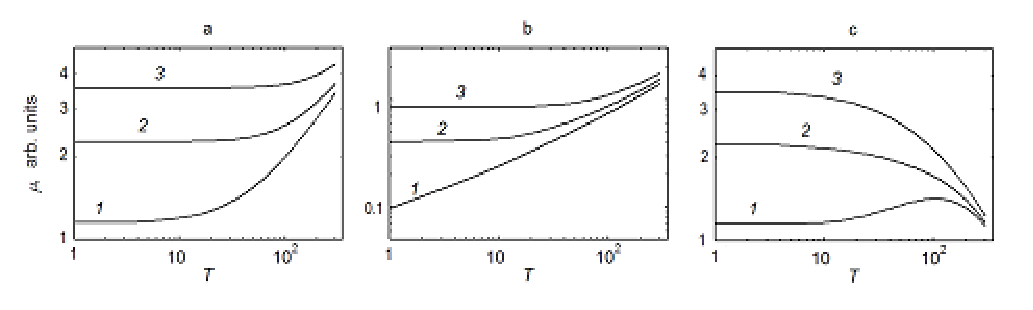
\includegraphics [scale=1] {image31}
	\captionsetup{labelformat=empty}
	\caption{Рис.  Температурная зависимость подвижности (в относительных единицах): a -- при учете рассеяния носителей на шероховатой поверхности в КЯ при $\Lambda =70 \AA$, $\Delta =3 \AA$, $L_{0} = 100 \AA$, кривые 1, 2, 3 получены соответственно для $n_{s} = 10^{11} \text{cm}^{-2}$, $n_{s} = 7 \cdot 10^{11} \text{cm}^{-2}$,$n_{s} = 1.5 \cdot 10^{12} \text{cm}^{-2}$; b -- при учете рассеяния носителей на шероховатой поверхности в КП при $\Lambda =20 \AA$, $\Delta =2 \AA$, $R_{0}=100 \AA$, кривые 1, 2, 3 получены соответственно для $n_{l} = 10^{5} \text{cm}^{-1}$, $n_{l} = 5 \cdot 10^{5} \text{cm}^{-1}$,$n_{s} = 10^{6} \text{cm}^{-1}$; c -- при учете рассеяния носителей на шероховатой поверхности и на фононах в КЯ при $\Lambda =70 \AA$, $\Delta =3 \AA$, $L_{0}=100 \AA$, кривые 1, 2, 3 получены соответственно для $n_{s} = 10^{11} \text{cm}^{-2}$, $n_{s} = 7 \cdot 10^{11} \text{cm}^{-2}$,$n_{s} = 1.5 \cdot 10^{12} \text{cm}^{-2}$} 
	\label{img:fig_3_1_1} 
\end{figure}

\section{ Электропроводность в размерно-квантовых системах с учётом рассеяния носителей на шероховатой поверхности в магнитном поле}

Рассмотрим особенности электропроводности, возникающие в размерно-квантованных системах в присутствии однородного магнитного поля напряжённостью $\vect{H}$. Для параболических КЯ в продольном магнитном поле ($\vect{H} || OX$) электропроводность для основного состояния описывается соотношением:
\begin{equation} \label{eq:32_10}
\sigma _{xx} =\frac{e^{2} \hbar ^{3} n}{m^{2} \gamma V_{0}^{2} } \left[\frac{\omega }{\Omega } \right],
 \end{equation}
\[
\Omega ^{2} =\omega ^{2} +\omega _{c}^{2},
\] 
\[
\hbar \omega =\frac{1}{L} \left(\frac{8\Delta E_{c} }{m} \right)^{\frac{1}{2} } 
\]
-- шаг пространственного квантования, $\omega _{c} $-- циклотронная частота, $n$-- концентрация носителей.

\begin{equation} \label{eq:32_20}
V_{0} =\frac{\hbar }{2} \left(\frac{\omega }{\Omega } \right)\frac{\partial \omega }{\partial L} .
\end{equation}

С учётом \eqref{eq:32_10}, \eqref{eq:32_20} подвижность для электронного газа с произвольным вырождением принимает вид:

\begin{equation} \label{eq:32_30}
\mu _{xx} =\frac{4e\hbar }{m^{2} \gamma } \left(\frac{\partial \omega }{\partial L} \right)^{-2} \left[1+\left(\frac{\omega _{c} }{\omega } \right)^{2} \right]^{\frac{1}{2} }.
\end{equation}

Заметим, что подвижность в размерно-ограниченных системах при учёте рассеяния носителей на длинноволновых колебаниях с ростом магнитного поля уменьшается \cite{Sinyavskii1998}. Это связано с ростом локализации зонных электронов. Как непосредственно следует из \eqref{eq:32_30} $\mu _{xx} $ с ростом магнитного поля увеличивается. Такое поведение зависимости подвижности от продольного магнитного поля может быть понято из следующих соображений. В параболической КЯ радиус локализации электрона $\lambda _{0} =\sqrt{\frac{\hbar }{m\Omega } } $ с ростом напряженности магнитного поля уменьшается, число носителей тока, рассеивающихся на шероховатой поверхности размерно-ограниченной системы, становится меньше, что и приводит к росту подвижности.

В поперечном магнитном поле в плоскости КЯ ($\vect{H} || OY$) матричные элементы обобщённого импульса, входящие в общее выражение для электропроводности \eqref{eq:31_150} определяются следующим образом:
\begin{equation} \label{eq:32_40}
P_{\alpha \beta }^{\left(x\right)} =\hbar k_{x} \left(\frac{\omega }{\Omega } \right)\delta _{\alpha \beta } -\frac{m\omega _{c} }{\sqrt{2} \lambda } \delta _{k_{x} k'_{x} } \delta _{k_{y} k'_{y} } \left\{\sqrt{n} \delta _{n,n_{1} +1} +\sqrt{n+1} \delta _{n,n_{1} +1} \right\}.
\end{equation}
Следовательно, матричный элемент обобщенного импульса имеет как диагональные элементы (первое слагаемое в \eqref{eq:32_40}) так и недиагональные элементы по квантовому числу размерно-магнитного квантования (второе слагаемое). Заметим, что диагональный матричный элемент возникает только в размерно-ограниченных системах (при $\omega \to 0$ это слагаемое в \eqref{eq:32_40} отсутствует).

В дальнейшем будем рассматривать электропроводность с учётом диагонального слагаемого в матричном элементе обобщенного импульса. Подвижность в поперечном магнитном поле при низких температурах для основного состояния имеет вид:
\begin{equation} \label{eq:32_50}
\mu _{x} =\frac{4e\hbar }{m^{2} \gamma } \left(\frac{\partial \omega }{\partial L} \right)^{-2} \left[1+\left(\frac{\omega _{c} }{\omega } \right)^{2} \right]^{-\frac{1}{2} }
\end{equation}
Следовательно, с ростом магнитного поля подвижность уменьшается и при $\left(\frac{\omega _{c} }{\omega } \right)^{2} >>1$ $\mu _{x} \sim \frac{1}{H} $. Такое поведение подвижности от $H$связано с тем, что в скрещенных магнитном и электрическом полях носители с дрейфовой скоростью перемещаются вдоль оси пространственного квантования по трохоиде, поэтому активно участвуют в процессах рассеяния на шероховатостях поверхности размерно-квантовой системы. 

Рассмотрим электропроводность в квантовых проволоках в однородном магнитном поле. В продольном магнитном поле время релаксации, определяемое \eqref{eq:31_140}, вычисляется обычным образом. В результате
\begin{equation} \label{eq:32_60}
\frac{1}{\tau _{\alpha } } =\frac{\gamma _{0} }{\hbar ^{3} } 2mV_{\alpha }^{2} \frac{1}{\left|k_{x} \right|} . 
\end{equation}

Электропроводность \eqref{eq:31_150} в рассматриваемой модели параболической КП принимает вид:
\begin{equation} \label{eq:32_70}
\sigma _{xx} =\frac{4\hbar e^{2} }{2\beta \pi sm\gamma _{0} } \sum _{n\nu }\frac{1}{V_{n\nu }^{2} } \ln \left[1+\exp \left\{\beta \xi _{n\nu } \right\}\right]
\end{equation}
\[
V_{\alpha } =\frac{4}{\left[4+\delta ^{2} \right]^{\frac{1}{2} } } \left[n+\frac{1}{2} +\frac{\left|\nu \right|}{2} \right]\frac{\partial (\hbar \omega )}{\partial R_{0} } .
\] 
При этом $\xi _{n\nu } $определяется из уравнения для химического потенциала параболической КП:
\begin{equation} \label{eq:32_80}
\sum _{n\nu }\int _{0}^{\infty }\frac{dx}{1+e^{x^{2} -\beta \xi _{n\nu } } } =\frac{\pi n_{e} }{2} \left(\frac{\hbar ^{2} \beta }{2m} \right)^{\frac{1}{2} } 
\end{equation}

Для невырожденного электронного газа из \eqref{eq:32_80} следует:
\[
\sum _{n\nu }e^{\beta \xi _{n\nu } }  =n_{e} \left[\frac{\pi \hbar ^{2} \beta }{2m} \right]^{\frac{1}{2} } .
\] 
И, следовательно, для основного размерно-квантового состояния ($n=\nu =0$) подвижность записывается в виде:
\begin{equation} \label{eq:32_90}
\mu _{x}^{\left(nd\right)} =\frac{eR_{0}^{4} \left[4+\left(\frac{\omega _{c} }{\omega } \right)^{2} \right]}{4\gamma _{0} \left(\Delta E_{c} \right)\sqrt{2m\beta \pi } } . 
\end{equation}
В случае вырожденного электронного газа из \eqref{eq:32_80} не трудно получить
\[
\sum _{n\nu }\sqrt{\xi _{n\nu } }  =\pi n_{e} \left[\frac{\hbar ^{2} }{2m} \right]^{\frac{1}{2} } .
\] 
и для основного электронного состояния ($n=\nu =0$) подвижность определяется соотношением:
\begin{equation} \label{eq:32_100}
\mu _{x}^{\left(d\right)} =\frac{e\pi \left[4+\left(\frac{\omega _{c} }{\omega } \right)^{2} \right]n_{e} \hbar R_{0}^{4} }{8m\gamma _{0} \left(\Delta E_{c} \right)} .
\end{equation}
 
Следовательно, в продольном магнитном поле, подвижность, увеличивается ($\mu _{x} \sim H^{2} $ ) и существенным образом зависит от радиуса квантовой проволоки ($\mu _{x} \sim R_{0}^{4} $). Если для невырожденного электронного газа  подвижность (21) увеличивается с ростом температуры, то для вырожденной размерно-квантовой проволоки подвижность при низких температурах не зависит от $T$. На рис. 1 представлена зависимость сопротивления (в относительных единицах) от напряженности магнитного поля с учетом рассеяния носителей на шероховатой поверхности (пунктирная линия).Сплошной линией представлена зависимость относительного сопротивления от магнитного поля для нанопроволок висмута с учетом рассеяния на поверхности и на акустических фононах именно, такая зависимость сопротивления от магнитного поля экспериментально наблюдалась в работе \cite{Nikolaeva2004}.

\begin{figure}[h] 
	\center
	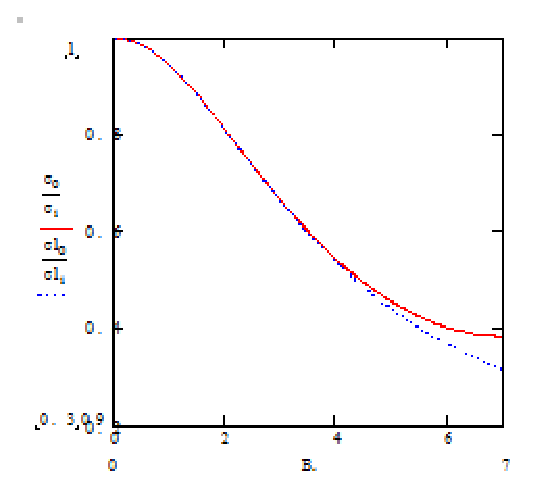
\includegraphics [scale=1] {image32}
	\captionsetup{labelformat=empty}
	\caption{Рис 1. Зависимость относительного сопротивления от магнитного поля для проволоки висмута ($d=80 \text{ nm}$, $T=4.2\text{ K}$). Пунктирной линией показана зависимость $R(H)/R(0)$ при учете рассеяния носителей на поверхности, сплошной линией при учете рассеяния носителей на поверхности и на акустических фононах.} 
	\label{img:fig_3_2_1} 
\end{figure}